\section{Criterio 4: ENERGIA}

Il criterio basato sull'energia prevede di calcolare l'energia totale della matrice mediante la seguente formula:

\begin{equation}
    Energia=\sum_{j=1}^r \sigma_j^2
\end{equation}

\noindent e di scegliere un numero k di valori singolari tale che 
\begin{equation}
    \sum_{j=1}^k \sigma_j^2
\end{equation}
sia almeno il 90\% dell'energia totale.\\

\noindent In questo caso l'energia totale della matrice è risultata essere 121874051. Volendo mantenere il 90\% dell'energia totale, ovvero 109686645.9,  il k suggerito è 94, con un energia pari a 109708426.061981
\begin{table}[H]
    \centering
    \begin{tabular}{|c|c|c|}
        \hline
        \textbf{Matrice} & \textbf{Righe} & \textbf{Colonne} \\
        \hline
        U\_troncata & 301 & 94 \\
        \hline
        S\_troncata & 94 & 94 \\
        \hline
        V\_troncata & 301 & 94 \\
        \hline
    \end{tabular}
    \caption{Dimensioni matrici troncate}
\end{table}

\begin{table}[H]
    \centering
    \begin{tabular}{|c|c|c|}
        \hline
        \textbf{Norma} & \textbf{Errore assoluto} \\
        \hline
        2 & 442.680374 \\
        \hline
        Frobenius & 3487.925592 \\
        \hline
    \end{tabular}
    \caption{Norme ed errori}
\end{table}

\noindent
E' noto inoltre che l'errore assoluto in norma due risulta essere $\sigma_{k+1}$ e in norma Frobenius 
\begin{equation}
    \sqrt{\sum_{i=k+1}^{r}\sigma_i^2}
\end{equation}
 dove k è il numero di valori singolari mantenuti.\\
Per la binarizzazione sono state utilizzate le seguenti soglie:
\begin{itemize}
    \item 0.25
    \item 0.5
    \item 0.75
    \item Soglia automatica calcolata con \textbf{graythresh}
\end{itemize}

\begin{figure}[H]
    \centering
     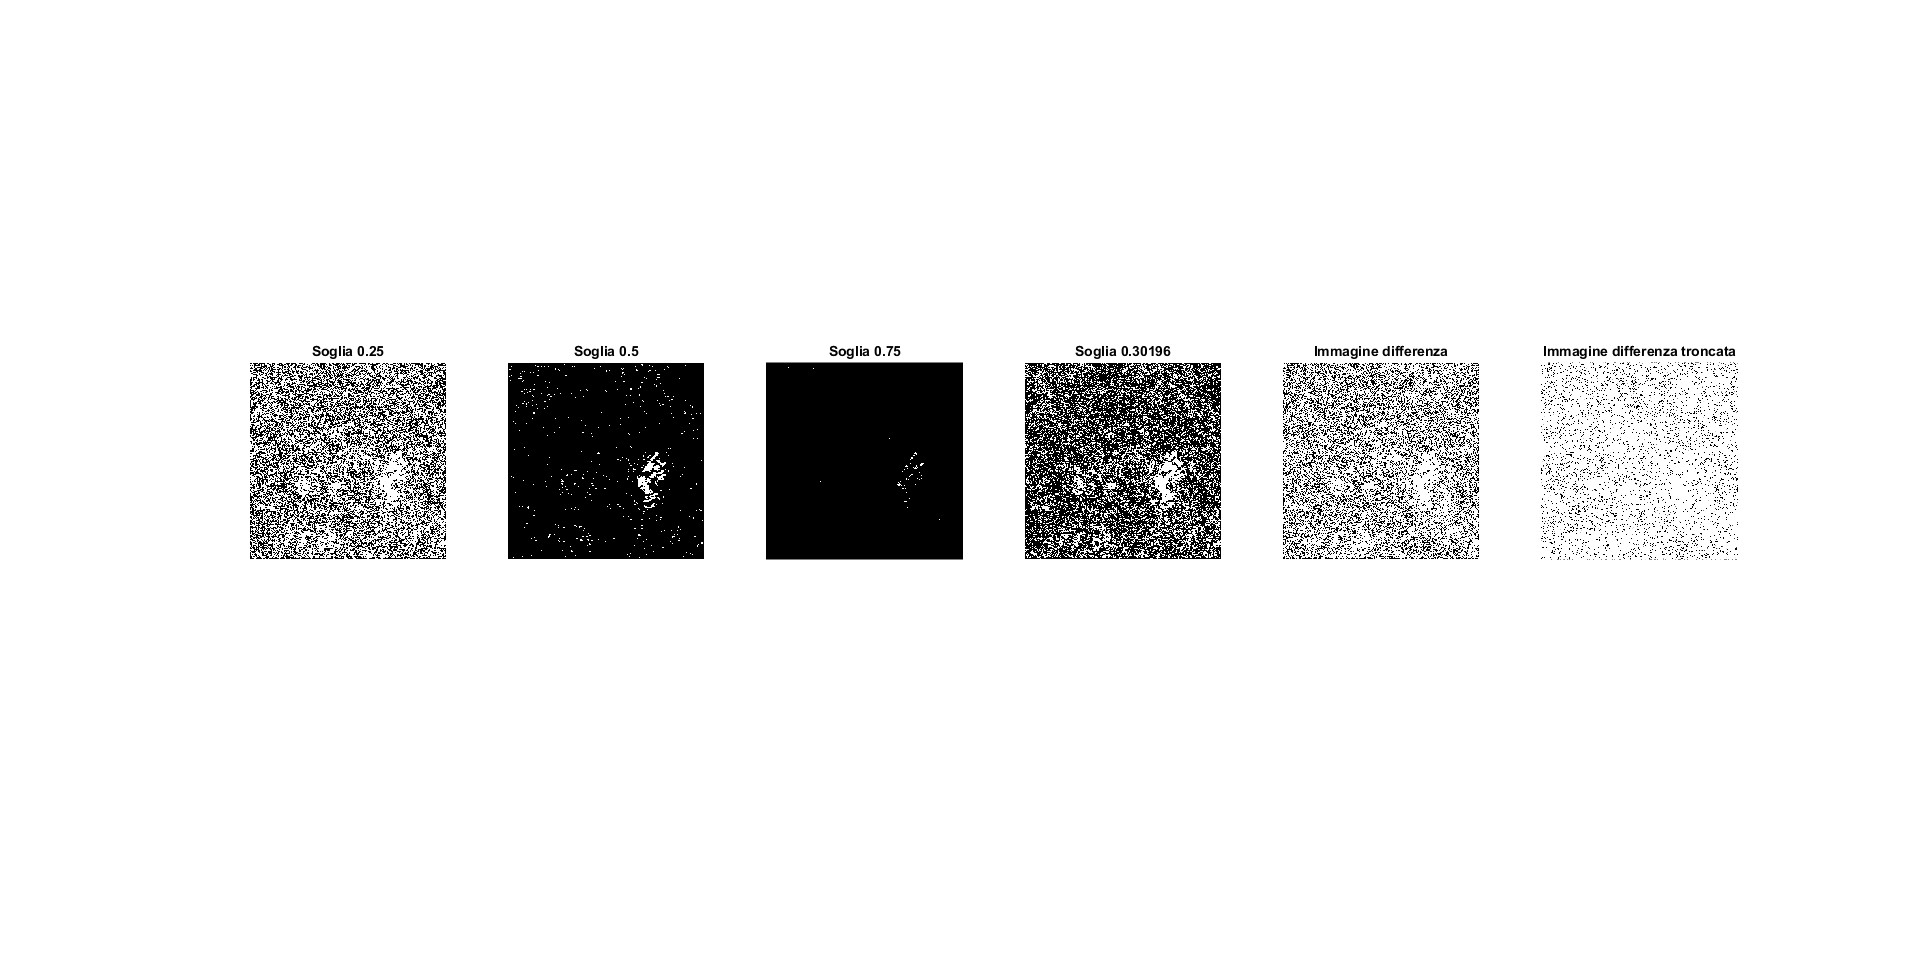
\includegraphics[width=\textwidth]{images/Criterio4.jpg}
    \caption{Immagini binarizzate con criterio 4}
\end{figure}

\noindent Le soglie 0.25 e automatica sono molto simili tra loro e sono "coerenti" sia con l'immagine originale che con quella troncata.

\noindent Per il processo di troncamento sono stati necessari in media circa \textcolor{blue}{\textbf{0.006}} secondi.\\



